
\documentclass[12pt,a4paper]{article}

% ============================================================
% INÍCIO DO PREÂMBULO
% ============================================================

% ---------- Bibliografia ----------
\usepackage[backend=biber, style=authoryear]{biblatex}
\addbibresource{references.bib}

% ---------- Codificação e idioma ----------
\usepackage[utf8]{inputenc}
\usepackage[T1]{fontenc}
\usepackage[brazil]{babel}

% ---------- Matemática ----------
\usepackage{amsmath, amssymb, amsfonts}

% ---------- Figuras e tabelas ----------
\usepackage{graphicx}
\usepackage{booktabs}
\usepackage{array}
\usepackage{float}

% ---------- Código-fonte ----------
\usepackage{listings}

% ---------- Formatação ----------
\usepackage{geometry}
\usepackage{setspace}
\usepackage{enumitem}
\usepackage{microtype}
\usepackage{hyperref}

% ---------- Margens ----------
\geometry{
    left=3cm,
    right=2cm,
    top=2.5cm,
    bottom=2.5cm
}

% ---------- Espaçamento ----------
\onehalfspacing
\setlength{\parindent}{1.25cm}
\setlength{\parskip}{0.15cm}

% ---------- Links ----------
\hypersetup{
    hidelinks
}

% ---------- Configuração simples para trechos de código ----------
\lstset{
    basicstyle=\ttfamily\small,
    breaklines=true,
    frame=single,
    showstringspaces=false,
    tabsize=4
}

% ============================================================
% FIM DO PREÂMBULO
% ============================================================


% ============================================================
% INÍCIO DOS DADOS DO TRABALHO
% ============================================================

\title{
    \textbf{Trabalho Prático I}\\
    Fundamentos de Inteligência Artificial\\
    Problema da Ponte e da Tocha
}

\author{
    % --------------------------------------------------------
    % PREENCHER COM OS NOMES DOS INTEGRANTES
    % --------------------------------------------------------
    Diogo Muzzi \\
    Paulo Gomes \\
    Pedro Pessoa Santos Brochado
}

\date{
    Universidade Federal de Minas Gerais\\
    Departamento de Engenharia Elétrica\\
    2026
}

% ============================================================
% FIM DOS DADOS DO TRABALHO
% ============================================================


\begin{document}

% ============================================================
% INÍCIO DA CAPA
% ============================================================

\maketitle
\thispagestyle{empty}

% ============================================================
% FIM DA CAPA
% ============================================================

\newpage

% ============================================================
% INÍCIO DO SUMÁRIO
% ============================================================

\tableofcontents

% ============================================================
% FIM DO SUMÁRIO
% ============================================================

\newpage


% ============================================================
% INÍCIO DA SEÇÃO 1 — INTRODUÇÃO
% ============================================================

% !TeX root = main.tex

\section{Modelagem do Problema}
\label{sec:modelagem}

Para resolver o problema por meio de algoritmos de busca, ele é modelado como
um Problema em Espaço de Estados \parencite{poole2010}. Isso exige a definição
de um conjunto de estados, um estado inicial, um conjunto de ações disponíveis
para cada estado, uma função sucessora que produz os estados alcançáveis a
partir de um estado e uma ação, e uma função objetivo que determina se um
estado é uma solução.

\subsection{Representação dos estados}

Cada estado $s_i \in S$ é representado como uma tripla $s_i = (A, B, \alpha)$,
sendo:
\begin{itemize}
    \item $A$ o conjunto de pessoas do lado de origem da ponte;
    \item $B$ o conjunto de pessoas do lado de destino da ponte;
    \item $\alpha$ uma variável booleana que indica se a tocha está do lado
    $A$ (verdadeira) ou do lado $B$ (falsa).
\end{itemize}

Na implementação, essa tripla é acrescida de um quarto valor correspondente à
estimativa heurística do estado, utilizado apenas pela busca A* para
priorizar a expansão de estados mais promissores; esse valor não faz parte da
definição formal do estado e não influencia as demais buscas.

\subsection{Estado inicial e estado objetivo}

O estado inicial $s_0 = (P, \{\}, \text{true})$ representa a situação em que
todas as pessoas $P$ e a tocha estão do lado de origem, e o lado de destino
está vazio.

Um estado $s_i$ é considerado objetivo quando o lado de origem está vazio, o
lado de destino não está vazio e a tocha está do lado de destino, isto é,
$s_i = (\{\}, P, \text{false})$. É essa condição que o programa verifica para
determinar se a busca alcançou uma solução.

\subsection{Ações possíveis}

Em cada estado, a tocha se encontra em um dos dois lados da ponte, e apenas
pessoas desse mesmo lado podem se mover. As ações possíveis são a travessia de
uma ou duas pessoas do lado onde está a tocha para o lado oposto -- nunca mais
de duas, dada a capacidade da ponte. Chamamos essas ações de
$q \in \{\mathit{ir}, \mathit{voltar}\}$: $\mathit{ir}$ quando o movimento
ocorre de $A$ para $B$ (tocha em $A$), e $\mathit{voltar}$ quando ocorre de
$B$ para $A$ (tocha em $B$). Como a tocha é necessária para enxergar a ponte,
toda travessia -- de ida ou de volta -- desloca a tocha junto com as pessoas
que se movem, alternando seu lado a cada ação.

\subsection{Função sucessora}

A função sucessora tem assinatura $F(s_i, p_i, q_i)$, em que $q_i$ é o tipo de
ação ($\mathit{ir}$ ou $\mathit{voltar}$) e $p_i \subseteq P$ é o conjunto de
uma ou duas pessoas que atravessam a ponte a partir do estado $s_i$, sempre
pertencentes ao lado de onde a tocha parte. A função retorna o estado
resultante de transferir as pessoas de $p_i$ entre os lados $A$ e $B$ e de
inverter a posição da tocha:

\begin{equation}
\begin{cases}
F(s_i, p_i, q_i=\mathit{ir}) = (A \setminus p_i,\; B \cup p_i,\; \text{false})
\\
F(s_i, p_i, q_i=\mathit{voltar}) = (A \cup p_i,\; B \setminus p_i,\; \text{true})
\end{cases}
\end{equation}

Dado um estado, todos os seus sucessores são obtidos aplicando $F$ a cada
combinação possível de uma ou duas pessoas do lado onde está a tocha. Como a
mesma ação pode levar de volta a um estado já visitado (por exemplo, uma
pessoa que atravessa e depois retorna sozinha), a função sucessora não evita
ciclos: essa responsabilidade fica a cargo de cada algoritmo de busca, que
mantém um conjunto de estados já visitados para não reexpandi-los.

\subsection{Custos das transições}

O custo de uma transição corresponde ao tempo gasto na travessia, que é
determinado pela pessoa mais lenta entre as que atravessam juntas -- já que
todas as pessoas do grupo cruzam a ponte no mesmo ritmo, limitado por quem
demora mais. Sendo $t(p)$ o tempo de travessia da pessoa $p$ e $M = p_i$ o
conjunto de pessoas que se movem em uma ação, o custo dessa transição é dado
por:

\[
c(M) = \max_{p \in M} t(p)
\]

\subsection{Representação do problema como grafo}

O espaço de estados pode ser visto como um grafo direcionado e ponderado, no
qual cada vértice corresponde a um estado $s_i \in S$ e cada aresta
corresponde a uma ação válida $F(s_i, p_i, q_i)$ que leva de um estado a
outro. O peso de cada aresta é o custo $c(M)$ da travessia associada. O grafo
é direcionado porque as ações de ida e de volta não são simétricas -- a tocha
precisa estar no lado de origem da ação -- e pode conter ciclos, já que é
possível retornar a um estado previamente visitado. Resolver o problema
corresponde, portanto, a encontrar um caminho no grafo entre o vértice que
representa o estado inicial $s_0$ e algum vértice que satisfaça a condição de
estado objetivo, sendo o caminho de menor custo total a solução ótima.


% ============================================================
% FIM DA SEÇÃO 2 — MODELAGEM DO PROBLEMA / TAREFA 1
% ============================================================


% ============================================================
% INÍCIO DA SEÇÃO 3 — BUSCAS NÃO INFORMADAS / TAREFA 2
% ============================================================

\section{Buscas Não Informadas}
\label{sec:buscas-nao-informadas}

Nesta etapa foram implementados dois métodos de busca não informada: 
a Busca em Profundidade (\textit{Depth-First Search} ou DFS) e a Busca 
em Largura (\textit{Breadth-First Search} ou BFS). Esses algoritmos exploram o 
espaço de estados utilizando apenas a estrutura de adjacência do 
grafo, sem levar em consideração o custo das arestas ou estimativas 
heurísticas sobre a proximidade do nó ao objetivo.

\subsection{Busca em Profundidade}
\label{subsec:dfs}

A Busca em Profundidade busca explorar o nó mais profundo (o mais longe do nó inicial) 
presente na fronteira de busca. Caso atinja um estado sem sucessores válidos não visitados, o 
algoritmo realiza o retorna para explorar ramos ainda não explorados.

Para implementar a política LIFO (\textit{Last-In, First-Out}) característica deste 
algoritmo, a fronteira foi estruturada por meio de uma pilha (\texttt{list} em Python). 
Cada entrada na pilha armazena uma tupla contendo o estado atual, a sequência de estados 
que compõem o caminho percorrido desde a raiz e o custo acumulado da trajetória.

Como o espaço de estados do problema da Ponte e da Tocha contém múltiplos ciclos 
(devido à possibilidade de pessoas realizarem travessias repetidas de ida e volta), 
a DFS pura em árvore entraria em laços infinitos. Para garantir a terminação, foi 
adotada a busca em grafo com um conjunto de estados visitados (\texttt{visitados}). 
Um estado é formalmente adicionado a esse conjunto quando é retirado do topo da pilha 
para expansão. Caso um estado retirado já pertença a \texttt{visitados}, ele é descartado.

A cada iteração, verifica-se a condição de parada através do método 
\texttt{is\_estado\_final()}. Ao encontrar a configuração em que todas as pessoas e a 
tocha estão no destino, a busca é finalizada, retornando o 
caminho percorrido, o custo total associado e a quantidade de nós visitados. Além disso, 
a rotina aceita um parâmetro opcional \texttt{limite\_nos}, que encerra a exploração 
caso um número predeterminado de nós expandidos seja ultrapassado, protegendo a execução 
contra buscas excessivamente longas.

Embora a DFS possua complexidade de espaço vantajosa em árvores gerais, em problemas 
ponderados ela não oferece qualquer garantia de otimalidade. Como ela explora o 
primeiro ramo disponível até o nó folha, a solução encontrada frequentemente inclui 
movimentações redundantes e travessias demoradas, resultando em um tempo total de 
travessia muito superior ao mínimo possível.

\subsection{Busca em Largura}
\label{subsec:bfs}

A Busca em Largura explora o grafo em camadas de profundidade, expandindo 
todos os nós a uma distância de $d$ transições a partir do estado inicial antes de 
avaliar qualquer nó a distância $d+1$.

A política FIFO (\textit{First-In, First-Out}) foi implementada utilizando uma fila 
duplamente encadeada (\texttt{collections.deque}). Diferentemente da DFS, na BFS o 
registro no conjunto de visitados ocorre no momento em que os nós sucessores são gerados 
e enfileirados. Essa estratégia evita a inserção duplicada de estados idênticos em um 
mesmo nível na fronteira, economizando memória de forma substancial.

A condição de parada é testada no momento em que o nó é desenfileirado. Se o estado 
corresponder à meta, o algoritmo retorna a solução. Pela propriedade fundamental da BFS, 
o primeiro caminho encontrado até o objetivo é garantidamente aquele com o 
\textbf{menor número de ações (nós visitados)}, mas não necessariamente o com menor custo.
Como as travessias possuem custos diferentes (ditados pela pessoa 
mais lenta do movimento), um caminho com menor número de passos pode apresentar um custo 
acumulado significativamente mais alto do que um caminho alternativo com o mesmo número 
de passos ou passos adicionais que sincronize melhor os tempos dos indivíduos.

% ============================================================
% FIM DA SEÇÃO 3 — BUSCAS NÃO INFORMADAS / TAREFA 2
% ============================================================
% ============================================================
% FIM DA SEÇÃO 3 — BUSCAS NÃO INFORMADAS / TAREFA 2
% ============================================================


% ============================================================
% INÍCIO DA SEÇÃO 4 — BUSCAS COM CUSTO E HEURÍSTICA / TAREFA 3
% ============================================================

\section{Busca de Custo Mínimo e Busca A*}

Nesta etapa foram implementados dois algoritmos que utilizam o custo das
transições para orientar a exploração do espaço de estados: a Busca de Custo
Mínimo e a Busca A*. Como o objetivo do problema da Ponte e Tocha é minimizar
o tempo total necessário para que todas as pessoas atravessem a ponte, o custo
acumulado até cada estado passa a ser uma informação essencial para a busca.

% ------------------------------------------------------------
% INÍCIO — FUNÇÃO DE CUSTO
% ------------------------------------------------------------

\subsection{Função de custo acumulado}

Em cada travessia, uma ou duas pessoas podem atravessar a ponte. O custo da
ação corresponde ao tempo da pessoa mais lenta entre aquelas envolvidas no
movimento. Dessa forma, para um conjunto $M$ de pessoas que atravessam, o
custo da transição é definido por

\[
c(M)=\max_{p\in M} t(p),
\]

em que $t(p)$ representa o tempo necessário para a pessoa $p$ atravessar a
ponte.

A função $g(n)$ representa o custo total acumulado desde o estado inicial até
o estado $n$. Para um sucessor $n'$ de $n$, tem-se

\[
g(n') = g(n) + c(n,n').
\]

Assim, $g(n)$ corresponde ao tempo efetivamente gasto para alcançar determinada
configuração do problema.

% ------------------------------------------------------------
% FIM — FUNÇÃO DE CUSTO
% ------------------------------------------------------------


% ------------------------------------------------------------
% INÍCIO — BUSCA DE CUSTO MÍNIMO
% ------------------------------------------------------------

\subsection{Busca de Custo Mínimo}

A Busca de Custo Mínimo seleciona para expansão o estado que possui o menor
custo acumulado $g(n)$. Para isso, foi utilizada uma fila de prioridade
implementada por meio da estrutura \texttt{heapq} da biblioteca padrão do
Python.

Na implementação, cada elemento da fronteira armazena o custo acumulado, um
valor auxiliar de desempate, o estado correspondente e o caminho percorrido
até ele. Dessa forma, o elemento retirado da fila é sempre aquele associado ao
menor valor de $g(n)$.

Também foi utilizado um dicionário denominado \texttt{melhor\_custo}, que
armazena o menor custo conhecido para alcançar cada estado. Quando um sucessor
é gerado, calcula-se

\[
g(n') = g(n) + c(n,n').
\]

Caso esse novo valor seja menor que o custo anteriormente registrado para o
mesmo estado, o dicionário é atualizado e o novo caminho é inserido na fila de
prioridade.

Entradas antigas da fila, correspondentes a caminhos que já foram superados
por alternativas de menor custo, são descartadas durante a execução.

Como os custos das travessias são não negativos, quando o estado objetivo é
retirado da fila de prioridade, o custo associado a ele corresponde ao menor
custo possível para alcançar a solução.

% ------------------------------------------------------------
% FIM — BUSCA DE CUSTO MÍNIMO
% ------------------------------------------------------------


% ------------------------------------------------------------
% INÍCIO — FUNÇÃO HEURÍSTICA
% ------------------------------------------------------------

\subsection{Função heurística}

Para a Busca A* foi definida uma função heurística baseada no maior tempo de
travessia entre as pessoas que ainda permanecem no lado de origem da ponte.

A função utilizada é

\[
h(n)=
\begin{cases}
0, & \text{se a origem estiver vazia},\\[2mm]
\displaystyle\max_{p\in \mathrm{origem}(n)} t(p),
& \text{caso contrário}.
\end{cases}
\]

A ideia é considerar o tempo da pessoa mais lenta que ainda precisa sair do
lado inicial. Como todos os tempos de travessia são positivos, tem-se também

\[
h(n)\geq 0.
\]

Essa propriedade é compatível com a interpretação de $h(n)$ como uma
estimativa do custo restante. Entretanto, a condição essencial para garantir
que a heurística não comprometa a optimalidade do A* é a sua admissibilidade,
isto é, que ela nunca superestime o custo real mínimo até o objetivo.

A heurística é admissível porque a pessoa mais lenta que ainda se encontra na
origem obrigatoriamente precisará atravessar a ponte pelo menos uma vez antes
que o estado objetivo seja alcançado. Portanto, o custo real restante nunca
poderá ser menor que o tempo de travessia dessa pessoa.

Assim,

\[
h(n) \leq h^*(n),
\]

em que $h^*(n)$ representa o custo real mínimo restante entre o estado $n$ e
o objetivo.

A função também é consistente, isto é, para uma transição entre $n$ e $n'$,

\[
h(n) \leq c(n,n') + h(n').
\]

Em um movimento de ida, o custo da travessia é suficiente para cobrir uma
eventual redução da estimativa. Em um movimento de volta, pessoas são
adicionadas novamente ao lado de origem e, portanto, o maior tempo presente
nesse lado não diminui.

% ------------------------------------------------------------
% FIM — FUNÇÃO HEURÍSTICA
% ------------------------------------------------------------


% ------------------------------------------------------------
% INÍCIO — INTEGRAÇÃO DA HEURÍSTICA
% ------------------------------------------------------------

\subsection{Integração da heurística ao espaço de estados}

Para que a Busca A* utilize corretamente a função heurística, cada estado deve
armazenar uma estimativa correspondente à sua própria configuração.

No estado inicial, a heurística é calculada logo após a criação do estado. Nos
demais casos, primeiro é construído o estado sucessor, considerando as pessoas
movimentadas e a nova posição da tocha. Somente depois é calculado o valor da
heurística correspondente a esse novo estado.

Dessa forma, evita-se utilizar a estimativa de um estado anterior como se ela
pertencesse ao seu sucessor.

A função heurística padrão do projeto foi mantida com valor zero. Assim, o
espaço de estados pode continuar sendo utilizado por algoritmos que não
necessitam de informação heurística.

% ------------------------------------------------------------
% FIM — INTEGRAÇÃO DA HEURÍSTICA
% ------------------------------------------------------------


% ------------------------------------------------------------
% INÍCIO — BUSCA A*
% ------------------------------------------------------------

\subsection{Busca A*}

A Busca A* utiliza simultaneamente o custo acumulado e uma estimativa do custo
restante. Para cada estado é calculado

\[
f(n)=g(n)+h(n),
\]

em que

\[
g(n)
\]

representa o custo real já gasto para alcançar o estado, enquanto

\[
h(n)
\]

representa uma estimativa do custo restante até o objetivo.

A fila de prioridade do A* utiliza $f(n)$ para determinar qual estado será
analisado primeiro. Assim, diferentemente da Busca de Custo Mínimo, que utiliza
somente o custo acumulado, o A* também considera uma estimativa de quão próximo
o estado está do objetivo.

Na implementação, cada entrada da fila armazena o valor de prioridade, um
valor auxiliar de desempate, o custo acumulado $g(n)$, o estado e o caminho
percorrido.

O dicionário \texttt{melhor\_custo} continua armazenando apenas os valores de
$g(n)$, pois esses valores representam os custos reais conhecidos. Caso um
caminho de menor custo seja posteriormente encontrado para uma configuração já
conhecida, o estado pode ser inserido novamente na fila.

Como o objeto que representa um estado também contém o valor da heurística,
foi utilizada como identificação lógica da configuração a tupla

\[
(\text{origem},\text{destino},\text{posição da tocha}).
\]

Essa escolha evita que duas configurações equivalentes sejam interpretadas
como estados distintos apenas por apresentarem valores diferentes no campo da
heurística.

% ------------------------------------------------------------
% FIM — BUSCA A*
% ------------------------------------------------------------


% ------------------------------------------------------------
% INÍCIO — TESTES E RESULTADOS
% ------------------------------------------------------------

\subsection{Testes e validação da implementação}

Foram utilizados diferentes conjuntos de tempos de travessia para verificar o
funcionamento dos algoritmos. Os custos obtidos pela Busca de Custo Mínimo e
pela Busca A* foram comparados, verificando-se que ambos encontraram os mesmos
custos ótimos.

Os resultados utilizados durante a validação são apresentados na
Tabela~\ref{tab:testes-tarefa3}.

\begin{table}[H]
    \centering
    \caption{Custos encontrados nos testes da Tarefa 3.}
    \label{tab:testes-tarefa3}
    \begin{tabular}{ccc}
        \toprule
        Tempos de travessia & Busca de Custo Mínimo & Busca A* \\
        \midrule
        $[1]$ & 1 & 1 \\
        $[1,2]$ & 2 & 2 \\
        $[1,2,5]$ & 8 & 8 \\
        $[1,2,5,10]$ & 17 & 17 \\
        $[2,2,2]$ & 6 & 6 \\
        \bottomrule
    \end{tabular}
\end{table}

Para a instância clássica do problema,

\[
[1,2,5,10],
\]

os dois algoritmos encontraram uma solução de custo total igual a

\[
17 \text{ minutos}.
\]

Além da comparação dos custos finais, foram verificados os caminhos retornados
pelos algoritmos. Os testes confirmam que a posição da tocha é alternada após
cada movimento, que são movimentadas uma ou duas pessoas por travessia e que a
soma dos custos das transições coincide com o custo total informado pela
busca.

Também foi testada a Busca A* utilizando uma heurística nula,

\[
h(n)=0.
\]

Nesse caso,

\[
f(n)=g(n),
\]

fazendo com que o critério de prioridade do A* se torne equivalente ao da
Busca de Custo Mínimo. Os custos obtidos permaneceram iguais, servindo como
uma verificação adicional da implementação.

Os testes também verificaram o valor da heurística no estado inicial, no estado
objetivo e nos estados sucessores, além da propriedade de consistência nas
transições consideradas.

% ------------------------------------------------------------
% FIM — TESTES E RESULTADOS
% ------------------------------------------------------------


% ------------------------------------------------------------
% INÍCIO — CONSIDERAÇÕES DA TAREFA 3
% ------------------------------------------------------------

\subsection{Considerações sobre os métodos}

A principal diferença entre os dois algoritmos está no critério utilizado para
ordenar a fronteira.

Na Busca de Custo Mínimo,

\[
\text{prioridade}(n)=g(n),
\]

enquanto na Busca A*,

\[
\text{prioridade}(n)=g(n)+h(n).
\]

Assim, a Busca de Custo Mínimo considera somente o custo já realizado, enquanto
a Busca A* utiliza também informações específicas do problema para estimar o
custo que ainda falta.

Como a heurística escolhida é admissível, a Busca A* preserva a garantia de
encontrar uma solução ótima. Ao mesmo tempo, a informação heurística pode
orientar a exploração para regiões mais promissoras do espaço de estados.

A comparação quantitativa entre os quatro algoritmos utilizados no trabalho,
considerando custo da solução, número de nós expandidos e tempo de
processamento, será apresentada posteriormente na seção destinada à Tarefa 4.

% ------------------------------------------------------------
% FIM — CONSIDERAÇÕES DA TAREFA 3
% ------------------------------------------------------------

% ============================================================
% FIM DA SEÇÃO 4 — BUSCAS COM CUSTO E HEURÍSTICA / TAREFA 3
% ============================================================


% ============================================================
% INÍCIO DA SEÇÃO 5 — COMPARAÇÃO DOS ALGORITMOS / TAREFA 4
% ============================================================

\section{Comparação dos Algoritmos}
\label{sec:comparacao-algoritmos}
% ------------------------------------------------------------
% ESTA SEÇÃO DEVE ATENDER À TAREFA 4.
%
% O enunciado pede comparação dos quatro métodos:
% - DFS;
% - BFS;
% - Busca de Custo Mínimo;
% - A*.
%
% Comparar valores médios de:
% - custo da solução encontrada;
% - número de nós expandidos;
% - tempo de processamento.
%
% Também explicar:
% - por que BFS não garante menor tempo;
% - por que Custo Mínimo e A* garantem solução ótima.
% ------------------------------------------------------------
Nesta seção é apresentada a comparação experimental e teórica entre os quatro métodos 
de busca implementados: Busca em Profundidade (DFS), Busca em Largura (BFS), 
Busca de Custo Mínimo (UCS) e Busca A*. A análise contempla as métricas de qualidade da 
solução (custo total da travessia em minutos), esforço computacional de exploração 
(número de nós visitados/expandidos) e tempo de execução.

\subsection{Metodologia da comparação}
\label{subsec:metodologia}
% Explicar:
% - quantidade de execuções, se houver média;
% - instância utilizada;
% - forma de medir tempo;
% - definição adotada para "nó expandido";
% - eventual limite máximo de nós para DFS.
Os experimentos foram conduzidos sobre a seguint instância  do problema da Ponte e da 
Tocha, composta por quatro pessoas com os seguintes tempos individuais de travessia:

\[
P = \{A: 1\text{ min},\; B: 2\text{ min},\; C: 5\text{ min},\; D: 10\text{ min}\}.
\]

Como o espaço de estados desse problema é compacto e os tempos de busca individuais 
ocorrem na escala de frações de milissegundo, medições isoladas sofrem influência 
significativa de ruídos do sistema operacional (como escalonamento de processos e 
efeitos de memória cache) e da ordem de iteração em estruturas de conjunto 
(\texttt{set}) do Python. Para contornar essas flutuações, cada algoritmo foi executado 
ao longo de \textbf{100 repetições independentes}.

As métricas registradas foram:
\begin{enumerate}
    \item \textbf{Custo do caminho}: soma dos tempos das ações que compõem a solução encontrada, expressa em minutos ($g(s_{\text{objetivo}})$).
    \item \textbf{Nós visitados}: contagem de nós efetivamente retirados da fronteira de busca para teste de objetivo e expansão de sucessores.
    \item \textbf{Tempo de processamento}: tempo decorrido de CPU durante a execução da busca, medido em milissegundos (ms) por meio da função \texttt{time.perf\_counter()}.
\end{enumerate}

Todos os ensaios foram realizados em ambiente Linux x86\_64 com interpretador Python 3.13.

\subsection{Resultados}
\label{subsec:resultados}
% Inserir tabela final.
%
% Exemplo:
%
% \begin{table}[H]
%     \centering
%     \caption{Comparação entre os algoritmos de busca.}
%     \label{tab:comparacao-final}
%     \begin{tabular}{lccc}
%         \toprule
%         Algoritmo & Custo & Nós expandidos & Tempo (s) \\
%         \midrule
%         DFS & -- & -- & -- \\
%         BFS & -- & -- & -- \\
%         Custo Mínimo & -- & -- & -- \\
%         A* & -- & -- & -- \\
%         \bottomrule
%     \end{tabular}
% \end{table}

Os valores médios obtidos após as 100 execuções de cada algoritmo estão sumarizados na 
Tabela~\ref{tab:comparacao-final}.

\begin{table}[H]
    \centering
    \caption{Comparação das métricas médias obtidas ao longo de 100 repetições na instância $[1, 2, 5, 10]$.}
    \label{tab:comparacao-final}
    \begin{tabular}{lcccc}
        \toprule
        Algoritmo & Solução Ótima? & Custo Médio (min) & Nós Visitados & Tempo Médio (ms) \\
        \midrule
        Busca em Profundidade (DFS) & Não & 50{,}21 & 10{,}64 & 0{,}195 \\
        Busca em Largura (BFS) & Não & 29{,}66 & 26{,}00 & 0{,}390 \\
        Busca de Custo Mínimo (UCS) & Sim & 17{,}00 & 26{,}00 & 0{,}398 \\
        Busca A* & Sim & 17{,}00 & 26{,}00 & 0{,}408 \\
        \bottomrule
    \end{tabular}
\end{table}


\begin{figure}[H]
    \centering
    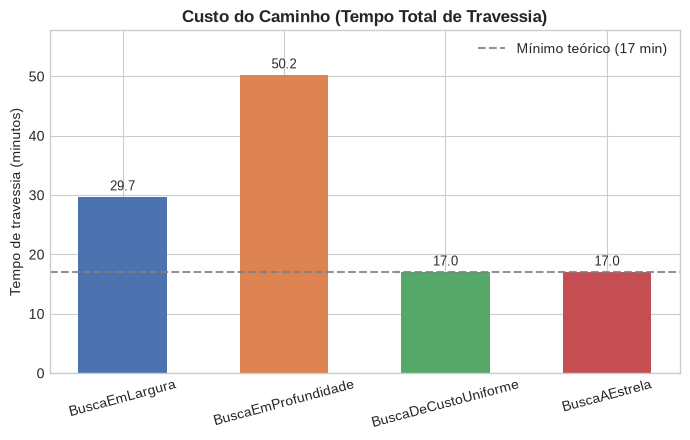
\includegraphics[width=0.75\textwidth]{results/grafico_custo.png}
    \caption{Comparação do tempo total de travessia (custo da solução) encontrado por cada algoritmo. A linha tracejada cinza indica o mínimo teórico ótimo de 17 minutos.}
    \label{fig:grafico-custo}
\end{figure}

\begin{figure}[H]
    \centering
    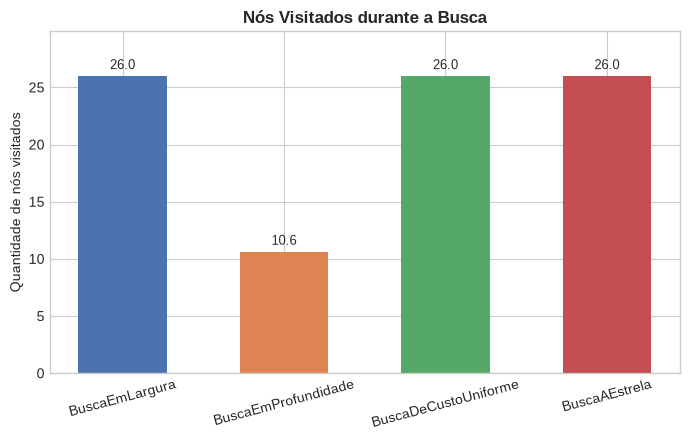
\includegraphics[width=0.75\textwidth]{results/grafico_nos_visitados.png}
    \caption{Quantidade média de nós visitados (expandidos da fronteira) até alcançar a solução.}
    \label{fig:grafico-nos}
\end{figure}

\begin{figure}[H]
    \centering
    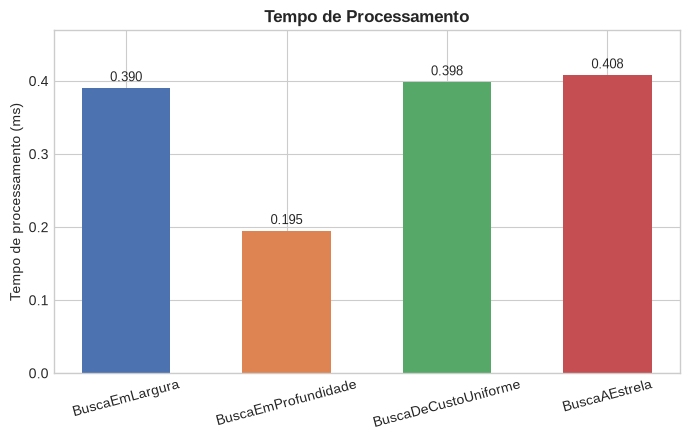
\includegraphics[width=0.75\textwidth]{results/grafico_tempo.png}
    \caption{Tempo médio de processamento por algoritmo expresso em milissegundos (ms).}
    \label{fig:grafico-tempo}
\end{figure}

\subsection{Discussão dos resultados}
\label{subsec:discussao}

% Discutir:
% - diferenças entre os algoritmos;
% - qualidade da solução;
% - quantidade de nós expandidos;
% - tempo de execução;
% - efeito da heurística no A*;
% - comportamento do DFS;
% - por que BFS não garante o menor tempo.
%
% Importante:
% Não apenas repetir os números da tabela.
% Interpretar os resultados.

A análise comparativa evidencia contrastes fundamentais na natureza e nas garantias 
oferecidas por cada família de algoritmos:

\begin{itemize}[leftmargin=1.5cm]
    \item \textbf{Busca em Profundidade (DFS)}: Apresentou o menor tempo médio de CPU 
    ($0{,}195\text{ ms}$) e a menor média de nós visitados ($10{,}64$). No entanto, esse 
    desempenho computacional aparece por ter encontrado uma solução sub-ótima mais cedo, 
    como vemos que o custo médio da travessia foi de $50{,}21\text{ minutos}$, quase três 
    vezes superior ao tempo ótimo. Por priorizar a profundidade, a DFS mergulha no 
    primeiro ramo exploratório disponível e tende a retornar a pessoas que já haviam 
    atravessado, gerando travessias repetitivas e selecionando pares arbitrários e 
    lentos. Trata-se, portanto, de um método inadequado quando o critério de sucesso 
    envolve a minimização do tempo de travessia.
    
    \item \textbf{Busca em Largura (BFS)}: Explorou exatamente $26{,}00\text{ nós}$ na 
    média, com tempo de execução de $0{,}390\text{ ms}$. A BFS cumpre estritamente sua 
    propriedade teórica de encontrar a solução com o \textbf{menor número de passos} 
    (5 travessias no total). Entretanto, o custo médio obtido foi de 
    $29{,}66\text{ minutos}$, consideravelmente acima do ótimo. Como a BFS é cega em 
    relação ao tempo dos participantes, ela frequentemente escolhe uma sequência de 
    5 passos que não emparelha os indivíduos mais lentos de forma estratégica.
    
    \item \textbf{Busca de Custo Mínimo (UCS)}: Encontrou o custo ótimo de 
    $17{,}00\text{ minutos}$ em 100\% dos ensaios, consumindo $0{,}398\text{ ms}$ e 
    visitando $26{,}00\text{ nós}$. Ao guiar sua fronteira pela função $g(n)$, 
    o algoritmo assegura que nenhum estado com custo acumulado superior a 17 seja 
    considerado antes do estado objetivo ideal.
    
    \item \textbf{Busca A*}: Também alcançou a solução ótima de 
    $17{,}00\text{ minutos}$, visitando $26{,}00\text{ nós}$ em $0{,}408\text{ ms}$. 
    A igualdade na quantidade de nós visitados entre A* e UCS decorre da dimensão 
    compacta do espaço de estados do problema: com 4 pessoas, o grafo possui no 
    total apenas 32 estados possíveis (dos quais 26 são alcançáveis até a profundidade 
    da solução). Como a estratégia ótima exige enviar as pessoas mais lentas juntas 
    ($C$ e $D$, gastando 10 min) e trazer de volta uma pessoa rápida ($A$ ou $B$), a 
    heurística $h_{\max}$, baseada exclusivamente na pessoa mais lenta remanescente na 
    origem, atinge seu valor máximo logo no início e não introduz podas adicionais no 
    reduzido volume de estados intermediários. Em instâncias com maior número de pessoas, 
    o A* passaria a podar significativamente mais estados do que a UCS graças ao 
    direcionamento fornecido por $h(n)$.
\end{itemize}

\subsection{Por que a Busca em Largura não garante a solução de menor tempo?}
\label{subsec:por-que-bfs-nao-garante-otimo}
% Explicar:
% - BFS minimiza profundidade / número de ações;
% - no problema, diferentes travessias têm custos diferentes;
% - menos movimentos não significa necessariamente menor tempo.
%
% Comparar com:
% - Custo Mínimo: ordena por g(n);
% - A*: ordena por g(n)+h(n), com heurística admissível.

A razão pela qual a Busca em Largura (BFS) não garante a solução ótima em tempo total 
decorre da diferença fundamental entre \textbf{otimação do número de arestas} e 
\textbf{otimação do custo do caminho (soma ponderada das arestas)}.

A BFS pressupõe que todas as arestas do grafo possuem custo idêntico ou unitário 
($c(u, v) = 1$). Sob essa premissa, o caminho com menor número de passos será
necessariamente o caminho de menor custo. Contudo, no Problema da Ponte e da Tocha, o 
grafo é ponderado com custos não uniformes determinados por $c(M) = \max_{p \in M} t(p)$,
o que faz com que encontre uma solução sub-ótima primeiro e por isso não explore outras
soluções alternativas.

No problema com $P = [1, 2, 5, 10]$, o número mínimo absoluto de travessias para levar 4 pessoas de um lado ao outro em uma ponte de capacidade 2 é de \textbf{5 passos} (três idas e duas voltas). Existem múltiplos caminhos distintos no grafo que alcançam o objetivo em exatamente 5 passos, por exemplo:

\begin{enumerate}
    \item \textbf{Caminho Subótimo em 5 passos}:
    \begin{itemize}
        \item Passo 1: $A$ e $D$ vão $\implies$ custo $\max(1, 10) = 10\text{ min}$.
        \item Passo 2: $A$ volta $\implies$ custo $1\text{ min}$.
        \item Passo 3: $A$ e $C$ vão $\implies$ custo $\max(1, 5) = 5\text{ min}$.
        \item Passo 4: $A$ volta $\implies$ custo $1\text{ min}$.
        \item Passo 5: $A$ e $B$ vão $\implies$ custo $\max(1, 2) = 2\text{ min}$.
    \end{itemize}
    Custo acumulado total: $10 + 1 + 5 + 1 + 2 = \mathbf{19\text{ minutos}}$ (ou valores ainda maiores, como 29 ou 37 min, se pessoas mais lentas retornarem com a tocha).

    \item \textbf{Caminho Ótimo em 5 passos}:
    \begin{itemize}
        \item Passo 1: $A$ e $B$ vão $\implies$ custo $\max(1, 2) = 2\text{ min}$.
        \item Passo 2: $A$ volta $\implies$ custo $1\text{ min}$.
        \item Passo 3: $C$ e $D$ vão juntos $\implies$ custo $\max(5, 10) = 10\text{ min}$.
        \item Passo 4: $B$ volta $\implies$ custo $2\text{ min}$.
        \item Passo 5: $A$ e $B$ vão $\implies$ custo $\max(1, 2) = 2\text{ min}$.
    \end{itemize}
    Custo acumulado total: $2 + 1 + 10 + 2 + 2 = \mathbf{17\text{ minutos}}$.
\end{enumerate}

Como ambos os caminhos possuem exatamente profundidade 5, ambos pertencem ao mesmo nível na árvore de busca da BFS. Como a BFS organiza sua fronteira exclusivamente pela ordem de chegada dos nós na fila FIFO, o primeiro estado objetivo desenfileirado dependerá unicamente da ordem arbitrária em que os sucessores foram gerados e inseridos na fila -- e não do tempo acumulado. Por isso, a BFS frequentemente retorna uma solução de 19, 29 ou mais minutos.

Em contrapartida, a \textbf{Busca de Custo Mínimo} organiza a fronteira em ordem crescente de $g(n)$, e a \textbf{Busca A*} organiza por $f(n) = g(n) + h(n)$. Sendo todos os custos de aresta não negativos e sendo a heurística $h(n)$ admissível (ou seja, $h(n) \leq h^*(n)$), ambos os algoritmos possuem a garantia matemática formal de que nenhum nó com custo real superior a 17 minutos será expandido antes que o caminho de custo mínimo seja selecionado, garantindo a solução ótima.

% ============================================================
% FIM DA SEÇÃO 5 — COMPARAÇÃO DOS ALGORITMOS / TAREFA 4
% ============================================================

% ============================================================
% INÍCIO DA SEÇÃO 6 — CONCLUSÃO
% ============================================================

\section{Conclusão}

% ------------------------------------------------------------
% SUGESTÃO:
%
% - Retomar o objetivo do trabalho.
% - Resumir o que foi aprendido com a comparação.
% - Comentar diferenças entre buscas informadas e não informadas.
% - Destacar a importância do custo e da heurística.
% - Não inserir novos resultados aqui.
% ------------------------------------------------------------

\textit{[Escrever aqui a conclusão geral do trabalho.]}

% ============================================================
% FIM DA SEÇÃO 6 — CONCLUSÃO
% ============================================================


% ============================================================
% INÍCIO DAS REFERÊNCIAS
% ============================================================

\printbibliography
% ============================================================
% FIM DAS REFERÊNCIAS
% ============================================================


% ============================================================
% INÍCIO DOS APÊNDICES — OPCIONAL
% ============================================================

% Descomente se o grupo quiser colocar códigos, tabelas grandes
% ou conteúdos auxiliares no final do documento.

% \appendix
%
% \section{Trechos adicionais de código}
%
% \begin{lstlisting}[language=Python]
% # Código adicional
% \end{lstlisting}

% ============================================================
% FIM DOS APÊNDICES
% ============================================================

\end{document}
